\documentclass[sigconf,review,anonymous]{acmart}

%% ---------------------------------------------------------------------------
%%  Architecture-as-Contract: A Substrate for Reviewable and Agentic
%%  Software Evolution in Monorepos.
%%  Initial draft targeting ACM FSE.
%% ---------------------------------------------------------------------------

\settopmatter{printacmref=true}
\setcopyright{none}
\renewcommand\footnotetextcopyrightpermission[1]{}

%% ----- Packages ------------------------------------------------------------
\usepackage{tikz}
\usepackage{pgfplots}
\pgfplotsset{compat=1.18}
\usetikzlibrary{positioning,arrows.meta,calc,fit,backgrounds,shapes.geometric,decorations.pathreplacing,shadows.blur}
\usepackage{booktabs}
\let\Bbbk\relax
\usepackage{amsmath,amssymb}
\usepackage{mathtools}
\usepackage{microtype}
\usepackage{enumitem}
\Urlmuskip=0mu plus 2mu\relax
\raggedbottom
\vfuzz=1.5pt

%% Define theorem environments explicitly (avoid relying on acmart option state).
\theoremstyle{plain}
\newtheorem{theorem}{Theorem}[section]
\newtheorem{lemma}[theorem]{Lemma}
\newtheorem{corollary}[theorem]{Corollary}
\newtheorem{property}[theorem]{Property}
\theoremstyle{definition}
\newtheorem{definition}[theorem]{Definition}
\newtheorem{assumption}{Assumption}

%% ----- A restrained, print-safe palette (Healy/Bostock sensibility) --------
%% Cool neutral ink, one warm accent for "danger/boundary", one cool accent
%% for "safe/interior". Backgrounds are desaturated washes, never saturated.
\definecolor{ink}{HTML}{1A1F24}        % near-black text/structure
\definecolor{slate}{HTML}{5B6B7A}      % secondary lines/labels
\definecolor{mist}{HTML}{E9EDF1}       % light fill for containers
\definecolor{mist2}{HTML}{D7DEE6}      % slightly darker container fill
\definecolor{steel}{HTML}{3D6A99}      % primary accent (safe / structural)
\definecolor{steelwash}{HTML}{E2EBF3}  % steel wash
\definecolor{rust}{HTML}{B5532A}       % warning accent (boundary / danger)
\definecolor{rustwash}{HTML}{F4E4DB}   % rust wash
\definecolor{moss}{HTML}{4E7A4E}       % "accepted / pass"
\definecolor{mosswash}{HTML}{E3EEE3}

%% ----- Shared TikZ styles --------------------------------------------------
%% Every figure draws from these so the paper has one visual language.
\tikzset{
  font=\sffamily,
  >=Stealth,
  %% nodes
  box/.style        = {rounded corners=2pt, draw=ink, line width=0.6pt,
                       fill=white, inner sep=5pt, align=center},
  container/.style  = {rounded corners=3pt, draw=slate, line width=0.6pt,
                       fill=mist, inner sep=8pt},
  leaf/.style       = {rounded corners=2pt, draw=steel, line width=0.6pt,
                       fill=steelwash, inner sep=4pt, align=center,
                       font=\sffamily\small},
  gate/.style       = {rounded corners=2pt, draw=ink, line width=0.7pt,
                       fill=white, inner sep=6pt, align=center},
  %% arrows
  dep/.style        = {->, draw=slate, line width=0.7pt},
  depnew/.style     = {->, draw=rust, line width=1.1pt},
  flow/.style       = {->, draw=ink, line width=0.8pt},
  agg/.style        = {-, draw=slate, line width=0.5pt, dotted},
  %% annotations
  lbl/.style        = {font=\sffamily\footnotesize, text=slate},
  caption/.style    = {font=\sffamily\small, text=ink},
}

\begin{document}

\title{Architecture as Contract: Typed Graphs
for Reviewable and Agentic Software Evolution}

\author{Anonymous Author(s)}
\affiliation{%
  \institution{Submitted for review}
  \country{}
}

\renewcommand{\shortauthors}{Anon.}

\begin{abstract}
Large repositories evolve through a steady stream of local edits, cross-cutting
refactorings, and, increasingly, changes proposed by coding agents. Human
review remains the main mechanism for protecting architectural intent, but the
artifact reviewers usually have is a textual diff. That diff is often a poor
proxy for the question reviewers actually need to answer: did this change alter
a module boundary, introduce a dependency, or widen an interface that other
parts of the system may rely on? Architecture diagrams express those concerns,
but in most projects they are informal drawings rather than checked artifacts
connected to the code.

We present \textsc{Archon}, a substrate for treating architecture as a
versioned, mechanically checked contract. \textsc{Archon} represents a
repository as a \emph{hierarchical attributed graph}: boxes nest from packages
down to functions, typed arrows record not only imports and calls but also
protocol fields, configuration keys, platform obligations, capabilities,
metrics, traces, and external runtime dependencies, and contracts state what
evidence is required at each boundary. The unit of review is a \emph{graph
delta} projected to the altitude at which the change should be understood,
together with an evidence-gap report: which boundaries changed, which contracts
are implicated, who should review them, and what tests, traces, proofs,
benchmarks, or human approvals are missing. We formalize the model, define node
identity across refactorings, and state a boundary-locality theorem: under
explicit assumptions about encapsulation and contract adequacy, an
implementation change with an empty boundary delta and a preserved behavioral
contract is unobservable outside the box. The theorem is not a claim that
current repositories satisfy these assumptions automatically; rather, it
identifies the checks and evidence needed to make autonomous internal evolution
defensible. \textsc{Archon} supports greenfield contract-first design and
brownfield snapshot-and-ratchet adoption, including instrumentation edits that
make previously unobservable invariants checkable.
\end{abstract}

\begin{CCSXML}
<ccs2012>
<concept><concept_id>10011007.10011006.10011008</concept_id>
<concept_desc>Software and its engineering~Software architectures</concept_desc>
<concept_significance>500</concept_significance></concept>
<concept><concept_id>10011007.10010940.10010992</concept_id>
<concept_desc>Software and its engineering~Software verification</concept_desc>
<concept_significance>300</concept_significance></concept>
<concept><concept_id>10011007.10011074.10011099</concept_id>
<concept_desc>Software and its engineering~Software evolution</concept_desc>
<concept_significance>500</concept_significance></concept>
</ccs2012>
\end{CCSXML}
\ccsdesc[500]{Software and its engineering~Software architectures}
\ccsdesc[500]{Software and its engineering~Software evolution}
\ccsdesc[300]{Software and its engineering~Software verification}

\keywords{software architecture, monorepos, dependency analysis,
architectural conformance, automated program evolution, code review}

\maketitle

%% ===========================================================================
\section{Introduction}
%% ===========================================================================

Engineers reason about software with boxes and arrows. A box is a unit of the
system: a service, a package, a class. An arrow is a dependency between two
units. This vocabulary underlies architecture whiteboards, onboarding talks, and
formal notations from UML package diagrams to the C4 model~\cite{c4model}. Yet
in many projects the picture remains a \emph{drawing}. It records intent, but it
is not mechanically connected to the code, and it can diverge from the system it
describes. The authoritative description of the architecture, namely what
actually imports, calls, or exposes what, is scattered through the source. It is
legible to compilers and language servers, but not in the form that a reviewer
or an automated proposer needs when evaluating architectural risk.

This gap matters more in large repositories. Monorepos make cross-cutting change
practical by placing many components in one versioned
space~\cite{potvin2016google,jaspan2018advantages}. The same affordance also
makes architectural erosion easy: a new import can cross a boundary that was
understood socially but never represented as an enforceable rule. Coding agents
add a second pressure. They can produce changes at the granularity of functions
or methods, often in large textual diffs whose architectural effect is small,
ambiguous, or accidentally broad. For both human and machine-authored changes,
the important review question is not simply how many lines changed. It is
whether the change alters a boundary that other parts of the system depend on.

The boundary is often not a source-level import. In systems such as LLM serving
engines, desktop application frameworks, and simulators, the review-relevant
fact may be that a pull request adds a sampling parameter, changes an IPC
permission, depends on a GPU backend, weakens a replay guarantee, removes an
observability field, or changes a minimum toolchain version. A practical
architecture substrate must therefore model \emph{operational} edges, not only
compiler edges, and it must report what evidence is missing when those edges
move. Otherwise it will be precise on toy module diagrams and unhelpful in the
repositories where reviewers most need it.

\paragraph{Thesis.}
We argue that the boxes-and-arrows view should become a \emph{first-class,
versioned, mechanically checked artifact}. We call that artifact
\textsc{Archon}, and design it to serve three related uses:
\begin{enumerate}[leftmargin=1.4em,itemsep=2pt,topsep=2pt]
\item \textbf{documentation}: a zoomable picture of the system derived from the
source rather than maintained separately;
\item \textbf{review}: a per-change \emph{architectural delta} that tells a
reviewer which boxes, arrows, and surfaces a pull request changes at the
altitude where that change is legible; and
\item \textbf{evolution}: the contract against which automated proposers are
checked before their changes are admitted.
\end{enumerate}
The useful observation is that these need not be three different systems. If the
same artifact documents the repository, defines the review delta, and supplies
the boundary checked for automated changes, then humans and tools share the same
architectural vocabulary.

\paragraph{Adoption constraint.}
For \textsc{Archon} to matter outside research prototypes, and for it to be
plausibly adoptable in CNCF-style infrastructure projects, it must be useful
before a repository is clean, fully specified, or ready for autonomous changes. We
therefore design for two adoption paths. In a \emph{greenfield} project, teams
can write the intended graph, contracts, and required evidence before or during
implementation. In a \emph{brownfield} project, \textsc{Archon} first snapshots
what exists, classifies which boundaries are real design commitments and which are
tolerated debt, and then ratchets through reviewed graph edits. The first useful
product is not a proof. It is a review-triage artifact: this change touched
these boundaries, implicated these contracts, needs these reviewers, and is
missing this evidence. Stronger automation grows only where that evidence has
been earned.

\paragraph{Approach.}
\textsc{Archon} represents a repository as a \emph{hierarchical attributed graph}
(\S\ref{sec:model}). Boxes nest along a containment tree---repository
$\supseteq$ package $\supseteq$ module $\supseteq$ function---and arrows are
typed. Some arrows are ordinary source dependencies; others represent protocol
fields, configuration variables, endpoint obligations, metrics, platform
targets, toolchain policies, or declared external systems. Coarse arrows are
defined as the \emph{aggregation} of the finer arrows beneath them
(Figure~\ref{fig:aggregation}). This single structure reconciles the two
granularities that the problem demands: humans review at the package altitude,
agents evolve at the function altitude, and the two are \emph{projections of the
same graph} rather than separate models that can drift apart. Each node carries
a \emph{structural contract}---its public surface and the typed arrows it is
permitted to have---and, where we intend to automate its evolution, behavioral
or operational obligations stated over that surface. Each obligation is
evidence-typed: structural check, unit or property test, replay trace,
differential oracle, benchmark, static check, or human approval. A change is
gated by its \emph{graph delta}, computed by extracting the graph before and
after and diffing the two; gating decisions are made per-altitude, so a change
that is a thousand-line internal rewrite at the function level can be
\emph{empty} at the package level and reviewed as such.

\paragraph{Pipeline justification.}
The model also makes explicit what must be true before internal automation can
be treated as low risk. We define node identity to be stable under the moves and
renames that refactoring and agents perform; otherwise a routine refactor would
appear as deletion plus creation and architectural deltas would be noisy. We
then state a boundary-locality result: if a change leaves a box's boundary delta
empty and preserves the box's behavioral contract, then, under explicit
assumptions about encapsulation and contract adequacy, the change is
unobservable to other boxes. The result is intentionally conditional: it does
not make automation safe by assertion, but identifies the facts the review
pipeline must establish. \textsc{Archon}'s contribution is to make those
preconditions visible in ordinary review: first establish that the boundary did
not move, then check or report the evidence needed to treat the implementation
as substitutable.

\paragraph{Separating the fixed from the open.}
A substrate for automated evolution should not depend on a particular agent or
search procedure. We therefore separate five concerns. Four form a \emph{fixed
substrate}: extraction, representation, structural conformance, and evidence
checking. The fifth is an \emph{open} space of \emph{proposers}: humans, coding
agents, and synthesis or search systems.
Every proposer emits the same kind of artifact, a graph delta plus a code
change, and is evaluated by the same gates. The point is not to predict which
proposer will be best, but to make the acceptance boundary independent of the
proposer.

\paragraph{Contributions.}
\begin{itemize}[leftmargin=1.4em,itemsep=3pt,topsep=2pt]
\item A \emph{hierarchical attributed graph} model of a repository that unifies
documentation, review, and agentic evolution as consumers of one versioned
artifact, with typed operational arrows and contracts that aggregate along a
containment tree (\S\ref{sec:model}).
\item A definition of \emph{node identity} stable under rename and move, which
makes architectural deltas signal rather than noise and makes ``the boundary
did not change'' computable (\S\ref{sec:identity}).
\item A \emph{pipeline justification} for fine-grained autonomous evolution
under coarse-grained human review: node identity, boundary deltas, evidence
obligations, and a boundary-locality theorem that states the assumptions under
which the Door-1 fast path is justified (\S\ref{sec:identity},
\S\ref{sec:guarantees}).
\item A \emph{conformance and evidence regime} of composable gates: acyclicity,
per-altitude spread, surface change, and evidence-gap reporting, together with
an evolution protocol that routes boundary-preserving changes to automated gates
and boundary-changing changes to human review of the delta
(\S\ref{sec:enforce},~\S\ref{sec:evolve}).
\item A practical \emph{adoption methodology} for both greenfield and brownfield
repositories: contract-first construction where possible, snapshot-and-ratchet
where necessary, and instrumentation edits as first-class architectural repairs
(\S\ref{sec:adoption}).
\item A concrete \emph{evaluation plan} across Go, Rust, and Python monorepos,
including review-triage studies, retrospective pull-request replay,
brownfield-repair studies, implementation case studies, and agentic evolution
experiments focused on behavioral-contract coverage
(\S\ref{sec:eval},~\S\ref{sec:agenda}).
\end{itemize}

This paper presents \textsc{Archon}'s model, the conditional guarantee it
supports, and the empirical plan needed to test whether the required assumptions
are practical in real repositories.

%% ===========================================================================
\section{Overview and Running Example}\label{sec:overview}
%% ===========================================================================

We draw our running example from \textsc{vLLM}~\cite{kwon2023vllm}, a
high-throughput LLM inference engine and a representative modern monorepo. Its
execution layer, the package \texttt{executor}, depends on its scheduling layer,
\texttt{core/sched}. Concretely, \texttt{Executor.execute\_model()} takes a
\texttt{SchedulerOutput} and \texttt{Executor.sample\_tokens()} takes a
\texttt{GrammarOutput}, both types defined in \texttt{core/sched}. At the
granularity an agent works in, these are distinct, type-driven import edges
among leaf entities (functions and classes). At the granularity a human reviews
in, they are a \emph{single} fact: \texttt{executor} depends on
\texttt{core/sched}. Figure~\ref{fig:aggregation} shows both views and the
relation between them. The package-level arrow is not a separate, hand-drawn
claim that might disagree with the code; it is the \emph{aggregation} of the
leaf-level edges, recomputed from the source on every change. This is the
property that keeps the documentation honest and the review legible at once.

Now suppose an evolution agent rewrites \texttt{execute\_model} to batch its
forward passes for throughput. At the leaf altitude this may be a large
implementation diff. At the package altitude it may be \emph{empty}: the set of
edges from \texttt{executor} to \texttt{core/sched} is unchanged, and the
function's signature is unchanged. We want a system in which
(i)~the reviewer can see that the cross-package architecture did not change, and
(ii)~the automated gate can distinguish this case from a rewrite that quietly
adds a dependency or widens an interface. If the relevant behavioral obligations
also hold, the system has a principled basis for treating the change as internal.
Sections~\ref{sec:model}--\ref{sec:guarantees} build this model; the present
section fixes intuitions and notation.

Throughout, we distinguish the \emph{actual} graph, extracted mechanically from
source and thus always faithful to the code, from the \emph{intended} graph, a
declared baseline that the actual graph is checked against. A pull request is
\emph{conformant} when the actual graph stays within what the intended graph
permits. For a greenfield repository, the intended graph may be written before
or alongside the first implementation. For a brownfield repository, which is the
more common and more difficult case, the intended graph is seeded by snapshotting
the actual graph (\S\ref{sec:enforce}); it then advances only through reviewed
deltas, so it encodes accumulated architectural intent without anyone having to
draw the whole architecture up front. This makes adoption descriptive before it
is prescriptive: first make the existing architecture visible, then decide which
future deltas are allowed.

%% ===========================================================================
\section{\textsc{Archon}'s Hierarchical Attributed Graph}\label{sec:model}
%% ===========================================================================

We model a repository state as a single artifact that carries structure
(boxes and arrows), hierarchy (boxes nest), and contracts (what each box
promises). We build it up in layers.

\subsection{Boxes, the containment tree, and arrows}

\begin{definition}[Architecture graph]\label{def:graph}
An \emph{architecture graph} is a tuple
$G = (V,\;\mathsf{par},\;E,\;\sigma)$ where
\begin{itemize}[leftmargin=1.4em,itemsep=1pt,topsep=2pt]
\item $V$ is a finite set of \emph{nodes} (boxes), each a unit of the system
at some altitude---repository, package, module/file, or leaf
(function, method, type, interface);
\item $\mathsf{par}:V \rightharpoonup V$ is a partial \emph{parent} map whose
graph is a rooted tree $T$ (the \emph{containment tree}): $\mathsf{par}(v)$ is
the box that directly contains $v$, undefined only at the root $r$;
\item $E \subseteq V \times \mathcal{K} \times V$ is a set of directed,
typed \emph{arrows}; the edge kind $k\in\mathcal{K}$ records whether the arrow
is, for example, an import, call, protocol field, configuration key, endpoint,
capability, metric, trace, platform target, toolchain policy, or external
runtime obligation; and
\item $\sigma$ assigns to each node its \emph{attributes}, including its
public surface and contracts (\S\ref{sec:contracts}).
\end{itemize}
We write $u \sqsubseteq v$ when $u$ is $v$ or a descendant of $v$ in $T$, and
$\mathsf{leaves}(v)=\{\ell : \ell \sqsubseteq v,\ \ell \text{ a leaf}\}$.
\end{definition}

The containment tree is what gives the model its two-altitude character: a
human reads a \emph{cut} of $T$ near the root (packages), an agent operates on
the leaves, and both are views of the same $V$.

\paragraph{Primitive edges are typed; coarse arrows are derived.}
Many primitive edges are compiler-visible facts: one leaf imports another,
calls another, reads a field, or implements an interface. Others are extracted
from schemas, build metadata, configuration files, permission manifests, trace
schemas, benchmark harnesses, or project policy files. A repository may also
declare \emph{external boxes} for dependencies that cannot be extracted with the
same precision: a GPU runtime, browser webview, model artifact, package
manager, cloud service, or adjacent repository. External boxes have surfaces
and declared contracts, but their internals are opaque. Formally $E$ is given at
the finest extracted or declared level, and arrows between interior boxes are
defined by \emph{aggregation}.

\begin{definition}[Arrow aggregation / projection]\label{def:agg}
For boxes $a,b \in V$ with $a \neq b$ and neither containing the other, the
typed \emph{aggregated arrow} $a \xRightarrow{k} b$ exists iff some leaf of $a$
has an edge of kind $k$ to some leaf of $b$:
\[
a \xRightarrow{k} b \quad\Longleftrightarrow\quad
\exists\, \ell_a \in \mathsf{leaves}(a),\ \ell_b \in \mathsf{leaves}(b)
\;:\; (\ell_a,k,\ell_b)\in E .
\]
The \emph{witness set} $W(a\!\xRightarrow{k}\! b)=\{(\ell_a,k,\ell_b)\in E :
\ell_a\sqsubseteq a,\ \ell_b\sqsubseteq b\}$ records the primitive edges the
arrow summarizes. The \emph{projection} of $G$ to an antichain $A\subseteq V$ of
$T$ (a set of boxes, no one containing another, covering all leaves) is the
typed graph on $A$ whose arrows are the aggregated arrows among members of $A$.
\end{definition}

Projection is the formal meaning of ``zoom'': choosing the antichain of all
packages yields the human's review diagram; choosing the antichain of all
leaves yields the agent's working graph. Because every coarse arrow carries its
witness set, the human can expand any arrow to see exactly which leaf
dependencies realize it (Figure~\ref{fig:aggregation}), and---crucially---a
change that does not alter $E$ within $W(a\!\xRightarrow{k}\! b)$ cannot alter
the typed arrow $a\!\xRightarrow{k}\! b$. The edge kind controls the evidence expected later:
changing a call edge is not the same review event as changing a permission edge,
a replay-trace edge, or a hardware-backend edge.

\subsection{Public surface and well-formedness}

A box hides its interior and exposes a surface. We make the surface explicit
because it, not the box's code, is what other boxes may depend on.

\begin{definition}[Public surface]\label{def:surface}
The \emph{public surface} $\mathsf{surf}(v)$ of a box $v$ is the set of its
entities (and their types/signatures) that are visible outside $v$. We require
graphs to be \emph{encapsulated}: every cross-box leaf edge enters its target
box through that box's surface. Formally, if $(\ell_a,k,\ell_b)\in E$ and the
nearest common ancestor of $\ell_a,\ell_b$ is a proper ancestor of $\ell_b$'s
parent box $b'$, then $\ell_b \in \mathsf{surf}(b')$.
\end{definition}

Encapsulation is what language mechanisms such as Go internal packages, Rust's
\texttt{pub(crate)} visibility, and Python's \texttt{\_\_all\_\_} conventions
approximate; an extractor can read these signals to compute
$\mathsf{surf}$. A graph is \emph{well-formed} if it is encapsulated and its
\emph{package-level projection satisfies the repository's cycle policy};
\S\ref{sec:enforce} discusses the strict acyclic policy used in the base model
and the empirical need to study migration paths for existing cyclic graphs.

%% ---- Figure 1: aggregation (real) ----------------------------------------
\begin{figure}[t]
\centering
%% Figure: arrow aggregation across two altitudes -- real vLLM example.
%% Column-width layout (fits ~241pt). executor depends on core/sched.
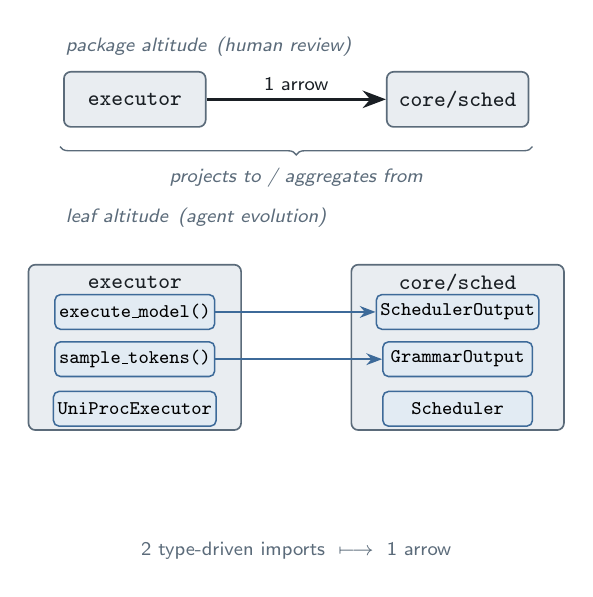
\begin{tikzpicture}[
  pkg/.style    = {rounded corners=2.5pt, draw=slate, line width=0.6pt, fill=mist, inner sep=4pt},
  leafn/.style  = {rounded corners=2pt, draw=steel, line width=0.55pt, fill=steelwash,
                   inner sep=1.5pt, align=center, font=\sffamily\fontsize{6.6}{7.6}\selectfont\ttfamily,
                   minimum width=19mm, minimum height=4.4mm},
  depagg/.style = {->, draw=ink, line width=1.2pt},
  fine/.style   = {->, draw=steel, line width=0.6pt},
  lbl/.style    = {font=\sffamily\scriptsize, text=slate},
  lblb/.style   = {font=\sffamily\footnotesize, text=ink},
]

%% ============ coarse (human) altitude ============
\node[lbl, anchor=west] at (-0.05,1.62) {\itshape package altitude \textcolor{slate}{\,(human review)}};
\node[pkg, minimum width=18mm, minimum height=7mm] (Pexec) at (0.95,0.95) {};
\node[lblb] at (Pexec.center) {\textbf{\texttt{executor}}};
\node[pkg, minimum width=18mm, minimum height=7mm] (Pcore) at (5.05,0.95) {};
\node[lblb] at (Pcore.center) {\textbf{\texttt{core/sched}}};
\draw[depagg] (Pexec.east) -- node[lbl, above, text=ink, yshift=-0.3mm] {1 arrow} (Pcore.west);

%% ============ projection brace ============
\draw[decorate, decoration={brace, amplitude=3pt, mirror}, slate, line width=0.5pt]
   (0.0,0.35) -- (6.0,0.35);
\node[lbl] at (3.0,-0.05) {\itshape projects to / aggregates from};

%% ============ fine (agent) altitude ============
\node[lbl, anchor=west] at (-0.05,-0.55) {\itshape leaf altitude \textcolor{slate}{\,(agent evolution)}};
\begin{scope}[yshift=-0.2cm]
  \node[pkg, minimum width=27mm, minimum height=21mm] (Ecl) at (0.95,-2.0) {};
  \node[lblb] at (Ecl.north) [yshift=-2.4mm] {\textbf{\texttt{executor}}};
  \node[leafn] (exec)   at (0.95,-1.55) {execute\_model()};
  \node[leafn] (sample) at (0.95,-2.15) {sample\_tokens()};
  \node[leafn] (uniproc)at (0.95,-2.78) {UniProcExecutor};

  \node[pkg, minimum width=27mm, minimum height=21mm] (Ccl) at (5.05,-2.0) {};
  \node[lblb] at (Ccl.north) [yshift=-2.4mm] {\textbf{\texttt{core/sched}}};
  \node[leafn] (sout)   at (5.05,-1.55) {SchedulerOutput};
  \node[leafn] (gout)   at (5.05,-2.15) {GrammarOutput};
  \node[leafn] (sched)  at (5.05,-2.78) {Scheduler};

  %% two parallel, non-crossing edges
  \draw[fine] (exec.east)   -- (sout.west);
  \draw[fine] (sample.east) -- (gout.west);
\end{scope}
\node[lbl] at (3.0,-4.78) {2 type-driven imports $\;\longmapsto\;$ 1 arrow};

\end{tikzpicture}

\caption{Aggregation across review altitudes. Two type-driven leaf imports
inside \textsc{vLLM}'s \texttt{executor} package aggregate to one package-level
arrow into \texttt{core/sched}. The arrow carries the witness set of leaf edges
it summarizes, so a change that does not touch those edges cannot change the
package-level arrow.}
\Description{A two-level architecture graph showing two executor leaf imports
into scheduler leaf types aggregating into one package-level executor to
core/scheduler arrow.}
\label{fig:aggregation}
\end{figure}

\subsection{Contracts: structural and behavioral}\label{sec:contracts}

Attributes $\sigma(v)$ carry two contracts per box, and optionally one per
arrow. Contracts are paired with \emph{evidence obligations}: the kind of
artifact required before a change touching the contract can be accepted.

\begin{definition}[Structural contract]
The \emph{structural contract} of a box $v$ is the pair
$\mathsf{SC}(v)=\big(\mathsf{surf}(v),\,\mathsf{Allow}(v)\big)$, where
$\mathsf{surf}(v)$ is its public surface and $\mathsf{Allow}(v)\subseteq V$ is
the set of typed targets $(k,u)$ that $v$ is permitted to depend on (its
allowed out-arrows by kind). A box \emph{satisfies} its structural contract when
its actual surface is a subset of the declared one and its actual out-arrows
target only allowed boxes by allowed edge kinds.
\end{definition}

\begin{definition}[Behavioral contract]\label{def:bc}
A \emph{behavioral contract} $\mathsf{BC}(v)$ of a box $v$ is a set of
properties over the observable behavior of $v$ \emph{at its public surface}:
predicates relating the inputs and outputs (and externally visible effects) of
the entities in $\mathsf{surf}(v)$. A behavioral contract may not refer to any
entity not in $\mathsf{surf}(v)$.
\end{definition}

\begin{definition}[Evidence obligation]\label{def:evidence}
An \emph{evidence obligation} is a pair $(p,\tau)$ attached to a box, arrow, or
surface element, where $p$ is the contract property and $\tau$ is the expected
evidence type. Evidence types include structural extraction, static analysis,
unit or property tests, fuzzing, replay traces, differential tests,
metamorphic tests, benchmarks, numerical tolerances, security or capability
checks, and explicit human approval.
\end{definition}

The surface-only restriction in Definition~\ref{def:bc} is deliberate and
load-bearing: a property that mentions a box's internals is not a contract but
a test of a particular implementation, and it would forbid exactly the internal
evolution we want to enable. Contracts at the surface are the obligations a
box's neighbors are entitled to rely on; everything else is free to change. We
return to this in \S\ref{sec:guarantees}, where it underwrites the safety
theorem. An \emph{arrow contract} on $a\!\xRightarrow{k}\! b$ is a consumer-driven
contract~\cite{fowler2006cdc}: the subset of $\mathsf{BC}(b)$ that $a$ actually
relies upon, which lets $b$ evolve freely so long as that subset holds.

Evidence obligations are what keep the methodology practical. A determinism
contract may require replay traces; a performance contract may require a
benchmark and confidence interval; a security/capability contract may require a
manifest check; a toolchain policy may require static metadata; and a design
change may require human approval. A missing obligation is not silently treated
as success. It becomes an \emph{evidence gap} surfaced in review.

\paragraph{Aggregating contracts up the tree.}
Arrows aggregate mechanically (Definition~\ref{def:agg}); contracts do not. We
\emph{state} a parent's behavioral contract independently at its own surface
rather than deriving it as the conjunction of its children's. Deriving it would
re-expose child internals at the parent boundary and forbid reorganizing
children---the opposite of what hierarchy is for. Thus $\mathsf{BC}(\textsf{package})$
constrains only the package's public surface, and the package's children may be
refactored arbitrarily as long as that surface contract continues to hold. This
asymmetry (arrows aggregate, contracts are restated) is a design decision we
revisit in \S\ref{sec:agenda}.

%% ===========================================================================
\section{Node Identity Under Refactoring}\label{sec:identity}
%% ===========================================================================

Everything downstream---legible diffs, the ``boundary unchanged'' check, the
safety theorem---rests on being able to say that a node \emph{after} a change
is ``the same node'' as one before, even though refactoring and agents
routinely rename entities and move them between files. If identity were keyed on
qualified path, then moving \texttt{execute\_model} from one executor file to
another would read as deleting one function and creating another: a maximal,
alarming delta for a no-op refactor, and worse, a spurious change to every
arrow incident on it. The delta would be noise, and ``the boundary did not
change'' would be uncomputable. We therefore make identity a first-class,
inferred relation rather than a syntactic key.

\begin{definition}[Identity correspondence]\label{def:identity}
Let $G,G'$ be the graphs before and after a change. An \emph{identity
correspondence} is a partial injection $\iota : V \rightharpoonup V'$ matching
nodes that denote the same architectural entity across the change. Nodes
outside $\mathrm{dom}(\iota)$ are \emph{deleted}; nodes outside
$\mathrm{range}(\iota)$ are \emph{created}; a matched pair $(v,\iota(v))$ is
\emph{renamed} if their names differ, \emph{moved} if their parents differ
(i.e.\ $\iota(\mathsf{par}(v)) \neq \mathsf{par}'(\iota(v))$), and
\emph{internally changed} if the leaf's body differs.
\end{definition}

We infer $\iota$ rather than trusting names, combining three signals in
decreasing order of authority:

\begin{enumerate}[leftmargin=1.4em,itemsep=2pt,topsep=2pt]
\item \textbf{Stable identifiers when available.} Some toolchains expose
durable symbol identifiers (e.g.\ a mangled symbol or a USR-style key) that
survive moves; when present they pin $\iota$ directly.
\item \textbf{Surface and signature match.} A leaf whose signature (name aside)
and incident edges are preserved is strong evidence of correspondence, even
across a rename.
\item \textbf{Tree-edit similarity.} For the residual, we match on structural
similarity of the entity's syntax tree using a fine-grained tree-differencing
algorithm in the style of \textsc{GumTree}~\cite{falleri2014finegrained},
thresholded to avoid coincidental matches.
\end{enumerate}

The contract that matters for the rest of the paper is the property $\iota$
must satisfy, not the particular heuristic used to compute it:

\begin{property}[Identity stability]\label{prop:identity}
A pure rename or move---a change that alters only $\mathsf{par}$ or the name of
a node, leaving its public signature, its body, and the set of edges incident
on it unchanged up to $\iota$---induces \emph{no} created or deleted nodes and
\emph{no} change to any aggregated arrow.
\end{property}

\noindent
Property~\ref{prop:identity} is what makes a refactor diff as a refactor.
\S\ref{sec:eval} treats the empirical accuracy of $\iota$ (its precision and
recall against developer-labeled refactorings) as a first-class research
question, since the value of every delta the system reports is bounded by it.
We are explicit about the failure mode: an \emph{incorrect} $\iota$ does not
threaten \emph{safety}---the structural and evidence gates still run on the
post-change graph regardless of how nodes were matched---but it degrades
\emph{legibility}, surfacing a clean refactor as a noisy delta. Safety depends
on the gates; identity governs only how clearly the change is presented and
whether it qualifies for the boundary-preserving fast path of
\S\ref{sec:evolve}.

%% ===========================================================================
\section{\textsc{Archon}'s Separation of Concerns}\label{sec:concerns}
%% ===========================================================================

\textsc{Archon}'s model of \S\ref{sec:model}--\ref{sec:identity} is realized by five
concerns (Figure~\ref{fig:substrate}). Four are a \emph{fixed substrate}; the
fifth is deliberately \emph{open}.

\begin{description}[leftmargin=*,itemsep=2pt,topsep=2pt,style=nextline]
\item[\textsf{1.\ Extraction} (language $\to$ graph)] Parses source into the
\emph{actual} graph---nodes at all altitudes, typed primitive edges, surfaces,
external boxes, and evidence metadata. This is the main ecosystem-specific
concern: Python, Go, Rust, build systems, permission manifests, trace schemas,
and CI metadata each require different extractors. Extraction reports facts and
decides no policy.
\item[\textsf{2.\ Representation} (the artifact)] The versioned hierarchical
graph: the single object all other concerns read. It stores structure and
contracts, not source, and must diff, address any node stably
(\S\ref{sec:identity}), and project to any altitude (Definition~\ref{def:agg}).
\item[\textsf{3.\ Conformance} (structural gate)] Given two graph versions and
the declared rules, emits the structural review report: acyclicity, spread,
surface, and typed-edge changes (\S\ref{sec:enforce}). Purely structural---fast,
total, deterministic.
\item[\textsf{4.\ Evidence} (contract gate)] Checks or records the evidence
obligations attached to implicated contracts: tests, fuzzing, traces,
benchmarks, static checks, or human approval. Grows lazily, per box and per
edge kind, as review needs and automation ambition grow.
\item[\textsf{5.\ Evolution} (proposers)] Anything that proposes a change: a
human, a coding agent, a synthesis or search system. \emph{Open by design.}
\end{description}

The discipline that makes the substrate reusable is stated as an invariant on
concern~5:

\begin{property}[Single funnel]\label{prop:funnel}
Every proposer's output is a pair (graph delta, code change), and a proposal is
accepted if and only if it passes the gates of concerns~3 and~4. No proposer
has any other path to acceptance.
\end{property}

\noindent
Property~\ref{prop:funnel} is what lets the substrate host evolutionary methods
that do not yet exist: a new agent framework can be placed in concern~5 without
changing concerns~1--4. Its proposals still encounter the same gates as
everyone else's. The gates are the contract between the repository and whatever
proposes changes to it.

%% ---- Figure 2: substrate (real) ----
\begin{figure}[t]
\centering
%% Figure: the five concerns -- fixed substrate vs. open proposers. Input by main.tex.
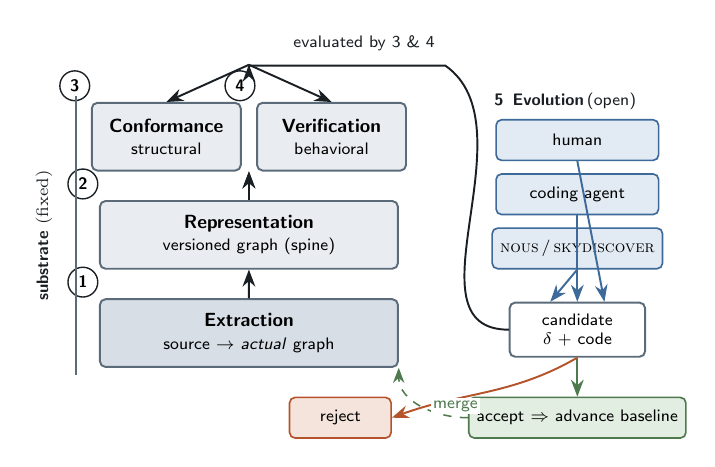
\begin{tikzpicture}[
  layer/.style = {rounded corners=2pt, draw=slate, line width=0.7pt,
                  minimum width=44mm, minimum height=10mm, align=center, fill=mist, font=\sffamily\footnotesize},
  num/.style   = {circle, draw=ink, line width=0.5pt, fill=white,
                  inner sep=0pt, minimum size=4.4mm, font=\sffamily\scriptsize\bfseries},
  prop/.style  = {rounded corners=2pt, draw=steel, line width=0.6pt, fill=steelwash,
                  minimum width=24mm, minimum height=6mm, align=center, font=\sffamily\scriptsize},
  gate/.style  = {rounded corners=2pt, draw=slate, line width=0.7pt, fill=white,
                  minimum width=20mm, minimum height=8mm, align=center, font=\sffamily\scriptsize},
  flow/.style  = {->, draw=ink, line width=0.7pt},
  lbl/.style   = {font=\sffamily\scriptsize, text=slate, align=left},
  scale=0.86, transform shape,
]

%% ---- substrate stack (left) ----
\node[layer, fill=mist2] (extract) at (0,0)
   {\textbf{Extraction}\\[0pt]{\scriptsize source $\to$ \emph{actual} graph}};
\node[layer] (repr) at (0,1.45)
   {\textbf{Representation}\\[0pt]{\scriptsize versioned graph (spine)}};
\node[layer, minimum width=22mm] (conf) at (-1.22,2.9)
   {\textbf{Conformance}\\[0pt]{\scriptsize structural}};
\node[layer, minimum width=22mm] (verif) at (1.22,2.9)
   {\textbf{Verification}\\[0pt]{\scriptsize behavioral}};

%% badges sit fully OUTSIDE the top-left corner so they never touch a title
\node[num] at ([xshift=-2.4mm,yshift=2.4mm]extract.north west) {1};
\node[num] at ([xshift=-2.4mm,yshift=2.4mm]repr.north west)    {2};
\node[num] at ([xshift=-2.4mm,yshift=2.4mm]conf.north west)    {3};
\node[num] at ([xshift=-2.4mm,yshift=2.4mm]verif.north west)   {4};

\draw[flow] (extract) -- (repr);
\draw[flow] (repr.north) -- (repr.north |- conf.south);
\draw[flow] (repr.north) -- (repr.north |- verif.south);

\draw[slate, line width=0.6pt] (-2.55,-0.62) -- (-2.55,3.5);
\node[lbl, rotate=90, anchor=south, text=ink] at (-2.78,1.44)
  {\itshape\bfseries substrate \normalfont(fixed)};

%% ---- proposers (right) ----
\node[lbl, text=ink, anchor=west] at (3.5,3.42) {\textbf{5\, Evolution}\,(open)};
\node[prop] (human)  at (4.85, 2.85) {human};
\node[prop] (agentA) at (4.85, 2.05) {coding agent};
\node[prop] (agentB) at (4.85, 1.25) {\textsc{nous}\,/\,\textsc{skydiscover}};

\node[gate, minimum width=20mm, minimum height=8mm] (cand) at (4.85,0.05)
   {candidate\\ $\delta$ + code};
\draw[flow, draw=steel] (human.south)  -- ([xshift=4mm]cand.north);
\draw[flow, draw=steel] (agentA.south) -- (cand.north);
\draw[flow, draw=steel] (agentB.south) -- ([xshift=-4mm]cand.north);

%% candidate -> gates 3 & 4: leave from the candidate's LEFT, run along a
%% clear corridor above the stack, then fork down into both gates. The corridor
%% (y=3.95) sits above every box and label, so the path clobbers nothing.
\coordinate (gap) at ($(conf.north east)!0.5!(verif.north west) + (0,0.55)$);
\draw[flow] (cand.west) to[out=180,in=-35] (2.9,3.95) -| (gap);
\draw[->, draw=ink, line width=0.7pt] (gap) -- (conf.north);
\draw[->, draw=ink, line width=0.7pt] (gap) -- (verif.north);
\node[lbl, text=ink, anchor=south] at (1.7,4.05) {evaluated by 3 \& 4};

%% verdicts
\node[prop, fill=mosswash, draw=moss, minimum width=24mm] (acc) at (4.85,-1.25)
   {accept $\Rightarrow$ advance baseline};
\node[prop, fill=rustwash, draw=rust, minimum width=15mm] (rej) at (1.35,-1.25) {reject};
\draw[flow, draw=moss] (cand.south) -- (acc.north);
\draw[flow, draw=rust] (cand.south) to[out=-150,in=20] (rej.east);
\draw[->, draw=moss, line width=0.55pt, dashed] (acc.west) to[out=180,in=-90] (extract.south east);
\node[lbl, text=moss, anchor=south, fill=white, inner sep=1pt] at (3.05,-1.2) {merge};
\end{tikzpicture}

\caption{Five concerns. Concerns 1--4 form a \emph{fixed} substrate;
concern~5---the proposers---is \emph{open}. Every proposer, human or machine,
emits the same artifact (a graph delta plus code) and is admitted only through
the same structural and evidence gates (Property~\ref{prop:funnel}).}
\Description{A pipeline diagram with extraction, representation, conformance,
and verification as fixed substrate layers, and human or machine proposers
feeding candidate graph deltas and code changes into those gates.}
\label{fig:substrate}
\end{figure}

%% ===========================================================================
\section{\textsc{Archon}'s Graph Delta and Structural Conformance}\label{sec:enforce}
%% ===========================================================================

A pull request transforms the actual graph from $G$ to $G'$. The unit of
review and gating is not the textual diff but the \emph{graph delta}.

\begin{definition}[Graph delta]\label{def:delta}
Given $G,G'$ and identity correspondence $\iota$ (\S\ref{sec:identity}), the
\emph{delta} $\Delta(G,G')$ is the labeled set of changes:
nodes created/deleted, nodes renamed/moved/internally-changed, arrows
added/removed/reversed by kind, surfaces widened/narrowed, and evidence
obligations added, discharged, or left missing---each computed up to $\iota$.
The \emph{delta at altitude $A$} (an antichain of $T$) is the delta of the
projections, $\Delta(\pi_A G,\ \pi_A G')$.
\end{definition}

The same physical change has different deltas at different altitudes
(\S\ref{sec:overview}): a leaf-body rewrite has a nonempty delta at the leaf
altitude and an \emph{empty} delta at the package altitude. This is precisely
what lets a large textual diff be reviewed as a small architectural one, and it
makes the reviewer's blast radius a measurable quantity rather than a
gut feeling.

\subsection{Four composable gates}

Conformance is the comparison of the actual graph against the intended baseline
$G_\star$ (seeded by snapshotting the actual graph at adoption; advanced only by
accepted deltas). We define four gates that cover cycles, change spread, public
surfaces, and evidence.

\paragraph{(G1) Acyclicity policy.}
In the base model, the package-level projection of $G'$ must be acyclic. Cycles
among packages collapse several modules into a single mutually dependent unit,
weakening the hierarchy the model relies on. The strict gate is cheap, requiring
a single topological sort of the package projection. For existing repositories
that already contain cycles, a practical implementation should either treat each
strongly connected component as a box or enforce a monotonic policy such as ``no
new cycles''; we include this migration question in the evaluation plan.

\paragraph{(G2) Spread --- per altitude.}
For each altitude $A$, the projected delta must touch no more than a budgeted
number of boxes and arrows:
\[
\begin{aligned}
\Delta_A &= \Delta(\pi_A G_\star, \pi_A G'),\\
|\text{boxes}(\Delta_A)| &\le \beta_A,\qquad
|\text{arrows}(\Delta_A)| \le \alpha_A .
\end{aligned}
\]
G2 is the formal answer to a common review pattern: a pull request may touch
dozens of files, boxes, and arrows, but still be self-contained at the package
altitude. Such a change can pass with a tight budget, while a genuine
cross-cutting change exceeds it and is \emph{routed to heightened review}, not
silently blocked. Budgets are per altitude because a change may legitimately be
broad at the leaf altitude (an agent rewriting one box) yet must be narrow at
the package altitude.

\paragraph{(G3) Surface --- per box.}
No box's public surface may grow relative to $G_\star$ without an explicit,
reviewed surface-widening in the delta. Surface narrowing is permitted only when
the delta also shows that no still-live external dependency is removed, or when
the affected callers are included in the same reviewed design change. G3 is what
makes ``the contract changed'' an event a human must approve, rather than an
accident hidden inside a textual diff.

\paragraph{(G4) Evidence --- per implicated contract.}
For every changed box, arrow, or surface element, \textsc{Archon} computes the contracts
whose scope includes that change and checks whether the required evidence
obligations (Definition~\ref{def:evidence}) have been discharged. G4 is not a
single pass/fail predicate in the same sense as acyclicity. It produces an
evidence status: \emph{satisfied}, \emph{missing}, \emph{stale}, or
\emph{human-review required}. This is the mechanism that turns the graph delta
into a practical review artifact: reviewers see not only what changed, but what
must be believed, tested, benchmarked, traced, or approved for the change to be
accepted.

\begin{definition}[Conformant change]\label{def:conformant}
A change $G \to G'$ is \emph{structurally conformant} iff $G'$ is well-formed
(\S\ref{sec:model}) and satisfies G1--G3 against $G_\star$. It is
\emph{evidence-complete} iff G4 reports no missing or stale obligation and no
unapproved human-review requirement. It is \emph{fully conformant} iff both
conditions hold.
\end{definition}

G1--G3 are independent and composed by conjunction; each is a total function of
$(G_\star, G', \iota)$ and so is deterministic and replayable in CI. Crucially,
they are \emph{structural}: they never run the program. This makes them cheap
enough to gate every push and is why they form the first line of the review
pipeline. G4 connects that structural result to the slower checks or human
approvals that the changed boundaries require.

%% ===========================================================================
\section{Adoption Methodology}\label{sec:adoption}
%% ===========================================================================

\textsc{Archon} is intended to be useful in repositories that are clean enough
to design deliberately and in repositories that are already messy. The same
artifact supports both, but the workflow differs.

\paragraph{Greenfield: contract-first construction.}
In a greenfield project, the intended graph $G_\star$ is written before or
alongside the first implementation. Teams declare boxes, public surfaces,
allowed typed arrows, external boxes, and evidence obligations while the design
is still cheap to change. Code then fills in the leaves. Every pull request is
reviewed against the same artifact the team used to design the system: if it
introduces a new endpoint, permission, toolchain constraint, backend target, or
configuration key, the graph delta makes that design choice visible. This path
is the strongest setting for the internal-evolution fast path
(\S\ref{sec:evolve}), because contracts and evidence can be attached before
agents are allowed to optimize internals.

\paragraph{Brownfield: snapshot, classify, ratchet.}
In a brownfield monorepo, the initial snapshot may contain cycles,
inappropriate dependencies, oversized boxes, missing observability, implicit
platform assumptions, and surfaces that grew through convenience rather than
design. Treating that snapshot as $G_\star$ does not endorse the mess; it
records the current contract so that new erosion is visible. Adoption proceeds
in four steps. First, extract and snapshot the actual graph. Second, classify
edges and surfaces as intended design, tolerated debt, or extractor uncertainty.
Third, install non-regression policies such as ``no new cycles,'' ``no new
dependence on this internal package,'' or ``no new public API without a graph
delta.'' Fourth, review a sequence of repair edits that move the baseline
toward a cleaner graph.

\paragraph{Repair edits.}
A repair edit is an intended graph edit plus an evidence obligation. Common
repairs include splitting a box, merging a strongly connected component into an
explicit larger box, introducing an adapter boundary, replacing a direct
dependency with an interface, removing an allowed arrow, narrowing a surface
after migrating callers, declaring an external box, or adding a missing
observability field. The last case is important: instrumentation is not merely
debugging support. If a contract cannot be checked until a trace field, metric,
event, or replay hook exists, then adding that observable fact is an
architectural repair.

\paragraph{Review-triage mode.}
The first deployment mode should not require complete formal safety. For a
large project, the immediately valuable output is a triage report: boundaries
touched, owners, contracts implicated, and evidence gaps.
For example, a change may touch a sampling-parameter boundary, a KV-transfer
path, and a backend-dispatch edge; it may implicate determinism and performance
contracts; and it may be missing a replay test or benchmark. Such a report is
useful even when the final decision remains human. It makes review routing,
test selection, and architectural discussion explicit, and it gives teams a
path from lightweight review aid to stronger automated gates as evidence
coverage improves.

\paragraph{Ordinary pull-request workflow.}
\textsc{Archon} should not ask authors to stop making ordinary pull requests.
Authors submit code, tests, documentation, migrations, and, when needed, a
design note or specification. The tool extracts $G'$ from the head revision and
computes the actual graph delta against the current baseline. If the boundary
delta is empty, the report should be small: the change is internal at the chosen
review altitude, the required evidence is satisfied or missing, and no
architecture review is required. If the boundary delta is nonempty, the report
becomes the review artifact: it names the boxes, arrows, surfaces, contracts,
evidence, and owners implicated by the PR. Authors may then attach the PR to an
existing design issue, create a graph amendment, or revise the code if the delta
was unintended. Appendix~\ref{app:workflow} spells out this lifecycle, including
specification-linked PRs, large tracking issues, and concurrent development.

\paragraph{Debt ratchets.}
Each repair edit creates a target graph $G_{\mathrm{target}}$ that is cleaner
than the current baseline according to an explicit policy, such as fewer package
cycles, lower fan-in to unstable internals, smaller public surfaces, fewer
cross-layer arrows, or greater observability for a contract. Code changes are
then evaluated against that target: a PR either realizes part of the repair,
leaves the debt unchanged, or moves the repository farther away and is routed to
review. This gives teams a ratchet rather than a flag day. The architectural
debt can be made visible immediately, but enforcement becomes stricter one
boundary, one SCC, one edge kind, or one evidence obligation at a time.

%% ===========================================================================
\section{\textsc{Archon} Evolution: Two Doors}\label{sec:evolve}
%% ===========================================================================

\textsc{Archon} admits exactly two kinds of change, distinguished by a single
predicate on the delta---\emph{does it touch any box boundary?}---and this
predicate determines which door a change goes through
(Figure~\ref{fig:doors}).

%% ---- Figure 3: the two doors (column-spanning) ----
\begin{figure*}[t]
\centering
%% Figure: the two doors -- decision flow on the boundary-delta predicate.
%% A clean left-to-right flow; the single branch is "empty boundary delta?".
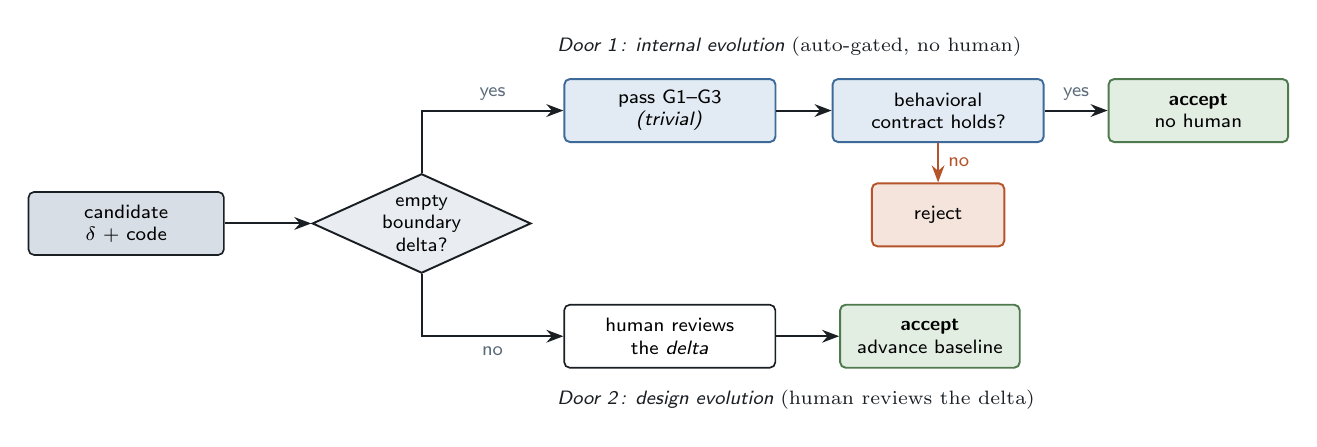
\begin{tikzpicture}[
  node distance=0pt,
  box/.style    = {rounded corners=2pt, draw=ink, line width=0.6pt, fill=white,
                   align=center, font=\sffamily\scriptsize, inner sep=4pt,
                   minimum height=8mm, text width=22mm},
  dec/.style    = {diamond, aspect=2.2, draw=ink, line width=0.7pt, fill=mist,
                   align=center, font=\sffamily\scriptsize, inner sep=1pt},
  gate/.style   = {rounded corners=2pt, draw=steel, line width=0.7pt, fill=steelwash,
                   align=center, font=\sffamily\scriptsize, inner sep=4pt,
                   minimum height=8mm, text width=24mm},
  term/.style   = {rounded corners=2pt, line width=0.7pt, align=center,
                   font=\sffamily\scriptsize, inner sep=4pt, minimum height=8mm, text width=20mm},
  flow/.style   = {->, draw=ink, line width=0.7pt},
  lbl/.style    = {font=\sffamily\scriptsize, text=slate},
  lblm/.style   = {font=\sffamily\scriptsize\itshape, text=ink},
  scale=1, transform shape,
]

%% start
\node[box, fill=mist2] (cand) at (0,0) {candidate\\ $\delta$ + code};

%% decision
\node[dec, right=11mm of cand] (dec) {empty\\ boundary\\ delta?};

%% ---- Door 1 (top): internal evolution, auto-gated ----
\node[gate, above right=7mm and 11mm of dec] (g1) {pass G1--G3\\ \emph{(trivial)}};
\node[gate, right=7mm of g1] (bc)  {behavioral\\ contract holds?};
\node[term, fill=mosswash, draw=moss, right=8mm of bc] (auto)
   {\textbf{accept}\\ no human};
\node[lblm, anchor=west] at (g1.north west |- g1.north) [yshift=4mm, xshift=-2mm] {Door 1\,: internal evolution \rmfamily\upshape(auto-gated, no human)};

%% ---- Door 2 (bottom): design evolution, human review ----
\node[box, below right=7mm and 11mm of dec, text width=24mm] (review)
   {human reviews\\ the \emph{delta}};
\node[term, fill=mosswash, draw=moss, right=8mm of review] (advance)
   {\textbf{accept}\\ advance baseline};
\node[lblm, anchor=west] at (review.south west) [yshift=-4mm, xshift=-2mm] {Door 2\,: design evolution \rmfamily\upshape(human reviews the delta)};

%% edges
\draw[flow] (cand) -- (dec);
\draw[flow] (dec.north) |- (g1.west) node[lbl, pos=0.75, above] {yes};
\draw[flow] (dec.south) |- (review.west) node[lbl, pos=0.75, below] {no};
\draw[flow] (g1) -- (bc);
\draw[flow] (bc) -- node[lbl, above] {yes} (auto);
\draw[flow] (review) -- (advance);

%% reject paths (subtle, downward)
\node[term, fill=rustwash, draw=rust, below=5mm of bc, text width=14mm] (rej1) {reject};
\draw[flow, draw=rust] (bc.south) -- node[lbl, right, text=rust] {no} (rej1.north);

\end{tikzpicture}

\caption{The two doors of evolution, selected by one predicate. A candidate
with an \emph{empty boundary delta} (Definition~\ref{def:bdelta}) is eligible
for Door~1: if the structural gates pass and the box's behavioral contract
holds, it may be accepted without human review. A candidate that touches any
boundary takes Door~2: its delta is reviewed by a human and, if approved,
advances the baseline. No proposer can reach the Door-1 fast path while
changing a boundary (Property~\ref{prop:doors}).}
\Description{A decision diagram in which a candidate graph delta and code change
is routed by whether its boundary delta is empty. Empty-boundary changes take an
automatic internal-evolution path; boundary-changing proposals take a human
design-review path.}
\label{fig:doors}
\end{figure*}

\begin{definition}[Boundary delta]\label{def:bdelta}
The \emph{boundary delta} of a box $v$ under $G \to G'$ is the restriction of
$\Delta(G,G')$ to $v$'s public surface and the arrows incident on $v$ (in or
out). It is \emph{empty} when $\mathsf{surf}(v)$, $\mathsf{Allow}(v)$, and the
witness sets of all arrows incident on $v$ are unchanged up to $\iota$.
\end{definition}

\paragraph{Door 1: internal evolution (auto-gated).}
A change whose boundary delta is empty for every box it touches changes only
box interiors, relative to the extracted model. It is eligible for automatic
admission if it (i)~is fully conformant (Definition~\ref{def:conformant}) and
(ii)~preserves the behavioral contracts of the boxes it touches, with the
required evidence discharged (concern~4).
This is the intended fast path for autonomous agents: an agent assigned the
interior of box $v$ may propose an implementation rewrite, and the gates check
that the proposal did not change the modeled boundary and did preserve the
surface obligations. \S\ref{sec:guarantees} states the assumptions under which
that is enough to justify accepting the change without human review.

\paragraph{Door 2: design evolution.}
A change with a nonempty boundary delta---a new box, a new arrow, a widened
surface, a new interface---alters the intended architecture. It produces a
graph delta that is \emph{itself} the reviewable artifact: a human (or a
higher-privilege policy) approves the \emph{delta}, which then advances the
baseline $G_\star$. Only after the boundary exists may Door-1 evolution fill in
the new box's interior.

Door~2 is also the normal path for evidence gaps. A proposal may be structurally
conformant yet missing the replay trace, benchmark, static check, or human
approval attached to an implicated contract. In that case \textsc{Archon} should not
pretend the change is safe or reject it without context. It routes the proposal
with an evidence-gap report, so maintainers can ask for the missing artifact,
approve an explicit exception, or revise the contract.

\begin{property}[Door separation]\label{prop:doors}
The two doors use the same artifact and the same gates; they differ only in
whether the boundary delta is empty. An empty boundary delta is necessary and
sufficient for the Door-1 fast path. Consequently no proposer can perform design
evolution while claiming internal evolution: a boundary-changing proposal
\emph{cannot} take the fast path, because the emptiness check fails.
\end{property}

\noindent
Property~\ref{prop:doors} is the operational core of the safety model. It
addresses a common failure mode of automation: an optimizer reports that it only
``tuned a function'' while adding a new dependency or widening an interface. In
our regime that proposal has a nonempty boundary delta and is routed through
Door~2, where the architectural change is visible.

%% ===========================================================================
\section{\textsc{Archon}'s Conditional Guarantee}\label{sec:guarantees}
%% ===========================================================================

We now make precise the conditional claim behind Door-1 evolution. The claim is
\emph{boundary locality}: a change confined to a box's interior, preserving its
contract, is unobservable to the rest of the system if interaction is mediated
through the box surface and the contract captures the observations contexts rely
on. The result is deliberately narrow. Its purpose is to state the acceptance
condition for internal rewrites in terms that a review pipeline can check or
report: boundary preservation is structural; behavioral preservation is an
evidence obligation.

\subsection{Observational model}

We treat each box $v$ as denoting a behavior $\llbracket v \rrbracket$: the
mapping from the inputs presented at its public surface to the outputs and
externally visible effects produced there. A \emph{context} $C[\cdot]$ for $v$
is the rest of the repository with a hole where $v$ sits; $C$ interacts with
$v$ \emph{only} through $\mathsf{surf}(v)$ and the arrows incident on $v$
(this is exactly what encapsulation, Definition~\ref{def:surface}, buys us).
Two boxes are \emph{observationally equivalent}, $v \approx v'$, if no
well-formed context can distinguish them:
$\forall C.\; \llbracket C[v] \rrbracket = \llbracket C[v'] \rrbracket$.

\begin{assumption}[Surface-mediated interaction]\label{asm:surface}
All interaction between a box and its context flows through the box's public
surface. Equivalently, the extractor's encapsulation (Definition~\ref{def:surface})
is sound: there is no hidden channel---no global mutable state, reflection, or
out-of-band file/network coupling---by which the context observes a box except
through $\mathsf{surf}(v)$.
\end{assumption}

\begin{assumption}[Adequate contract]\label{asm:adequate}
The behavioral contract $\mathsf{BC}(v)$ captures every surface behavior any
context relies upon: if $\mathsf{BC}(v)$ holds of two implementations, they are
interchangeable with respect to what surface observations contexts can make.
\end{assumption}

\noindent
We are deliberately explicit that these are assumptions, because they delimit
exactly where the guarantee can fail in practice---hidden channels
(Assumption~\ref{asm:surface}) and under-specified contracts
(Assumption~\ref{asm:adequate})---and \S\ref{sec:eval} and \S\ref{sec:agenda}
treat each as a measurable risk rather than a hope. Assumption~\ref{asm:surface}
is what the extractor must establish; Assumption~\ref{asm:adequate} is what
contract authoring (and its coverage) must establish.

\subsection{Boundary locality}

The theorem below packages the review obligation. The mechanically checkable
part is the empty boundary delta: same surface, same allowed arrows, same
witnesses. The evidence-dependent part is contract preservation. Where either
part is unavailable, \textsc{Archon} reports the gap instead of claiming safety.

\begin{theorem}[Boundary locality]\label{thm:locality}
Let a change transform box $v$ into $v'$ with an \emph{empty boundary delta}
(Definition~\ref{def:bdelta}) and suppose $v'$ satisfies $\mathsf{BC}(v)$. Then
under Assumptions~\ref{asm:surface}--\ref{asm:adequate}, $v \approx v'$: for
every well-formed context $C$, $\llbracket C[v] \rrbracket = \llbracket C[v']
\rrbracket$. In particular, no other box's behavior, and no aggregated arrow or
contract elsewhere in the graph, changes.
\end{theorem}

\begin{proof}[Proof sketch]
By Definition~\ref{def:bdelta}, an empty boundary delta gives
$\mathsf{surf}(v') = \mathsf{surf}(v)$, $\mathsf{Allow}(v')=\mathsf{Allow}(v)$,
and unchanged witness sets for all arrows incident on $v$. The interface the
context binds against is therefore identical. By Assumption~\ref{asm:surface}, any
context $C$ interacts with the hole solely through that interface, so $C$'s
observations of $v$ versus $v'$ are determined entirely by the surface
behaviors $\llbracket v\rrbracket,\llbracket v'\rrbracket$ restricted to
$\mathsf{surf}(v)$. Since $v$ satisfied $\mathsf{BC}(v)$ (it is the incumbent)
and $v'$ satisfies $\mathsf{BC}(v)$ by hypothesis, Assumption~\ref{asm:adequate}
gives that the two are indistinguishable under all surface observations a
context can make. Hence $\llbracket C[v]\rrbracket = \llbracket C[v']\rrbracket$
for all $C$, i.e.\ $v\approx v'$. Because aggregated arrows
(Definition~\ref{def:agg}) and arrow contracts are functions only of leaf edges
and surface behavior at the boundary---both unchanged---nothing elsewhere in
$G$ is affected.
\end{proof}

\begin{corollary}[Compositional autonomy]\label{cor:autonomy}
Door-1 changes to \emph{disjoint} boxes compose: if agents independently rewrite
the interiors of boxes $v_1,\dots,v_k$ with no two sharing a containment-ancestor
that is also rewritten, and each preserves its contract with an empty boundary
delta, then the combined change is observationally equivalent to applying them
in any order, and to the original.
\end{corollary}

\begin{proof}[Proof sketch]
Each rewrite is unobservable to its context by Theorem~\ref{thm:locality}; in
particular each is unobservable to the other rewritten boxes, which lie in the
context. Observational equivalence is a congruence under the well-formed
contexts here: replacing a well-formed box by an observationally equivalent box
preserves the surface and incident arrows through which any enclosing box can
observe it. Therefore the enclosing box is itself a valid context, and
independent equivalences compose and commute.
\end{proof}

\noindent
Theorem~\ref{thm:locality} justifies the protocol in \S\ref{sec:evolve}: the
structural check establishes that the modeled boundary did not change, and the
behavioral check establishes the obligations needed to treat the new
implementation as substitutable at that boundary.
Corollary~\ref{cor:autonomy} explains when such changes can be composed across
disjoint boxes. The structural check alone is not sufficient for behavioral
safety: it shows that the \emph{interface} did not move, not that
\emph{behavior} was preserved. Where a box has \emph{no} behavioral contract,
Door~1 still provides structural locality, but the behavioral claim degrades to
the ordinary evidence supplied by the box's tests. This is not a defect in the
theorem; it is the empirical frontier the evaluation must measure.

%% ===========================================================================
\section{Evaluation Plan}\label{sec:eval}
%% ===========================================================================

\textsc{Archon}'s claims require empirical support at five levels. First, the substrate
must be implementable for languages and ecosystems with different module,
visibility, configuration, policy, and runtime mechanisms. Second, graph deltas
and evidence-gap reports must be useful in real review histories, rather than
merely well defined. Third, the adoption workflow must work for both
contract-first greenfield projects and snapshot-and-ratchet brownfield projects.
Fourth, the algebra of graphs, deltas, projections, and gates must be tested as
software, not only specified on paper. Fifth, the Door-1 protocol must be tested
against agentic changes and independent behavioral oracles. We therefore plan
linked studies covering implementation, review triage, retrospective pull
requests, brownfield repair, executable invariants, and controlled agentic
evolution.

\paragraph{Subjects and case studies.}
We will study large open-source repositories spanning different levels of native
boundary enforcement and different kinds of review friction. Candidate subjects
include \textsc{vLLM}, a high-velocity Python/C++/Rust inference engine with
many hardware and API surfaces; BLIS, a Go inference-simulation codebase with
explicit behavioral invariants; and Tauri, a Rust/TypeScript application
framework organized around runtime, plugin, IPC, packaging, and platform
boundaries~\cite{vllmrepo,inferencesim,taurirepo,tauriarchitecture}. For each
repository we will also select two to four implementation case-study boxes:
components with nontrivial internal logic, a stable public surface, and enough
tests or specifications to support independent behavioral checking. These boxes
are the units on which behavioral contracts and agentic rewrites will be studied.

\paragraph{Research questions.}
The evaluation is deliberately asymmetric. The central claim is not that every
repository can be made safe for automation immediately. It is that a typed graph
and evidence report can improve review immediately, while identifying the
conditions under which automation becomes justified. We therefore organize the
study around four questions.

\begin{description}[leftmargin=2.6em,itemsep=3pt,topsep=2pt,style=sameline]
\item[\textbf{RQ1}] (Model extraction) What typed architecture graph can be
extracted with useful precision? We measure coverage for nodes, surfaces, typed
edges, external boxes, evidence metadata, and identity across refactorings. The
error analysis classifies dynamic imports, reflection, generated code, global
state, configuration, protocol fields, permission manifests, platform labels,
toolchain policies, and file or network channels.
\item[\textbf{RQ2}] (Review value) Do graph deltas and evidence gaps improve
ordinary review? For historical pull requests, we compare lines changed against
boxes, typed arrows, surfaces, implicated contracts, and evidence gaps; measure
empty package-level deltas; and test whether reports route changes to the same
owners, tests, specifications, and review discussions that maintainers
eventually used.
\item[\textbf{RQ3}] (Adoption and repair) Can teams adopt \textsc{Archon} before
their architecture is clean or fully specified? We compare greenfield use with
brownfield use, measuring time to first useful report, tolerated-debt
annotations, repair edits, instrumentation edits, plan-linked PRs, and whether
ratchets block changes maintainers consider routine.
\item[\textbf{RQ4}] (Door-1 automation) When does the internal-evolution fast
path preserve behavior? On case-study boxes with surface contracts, we ask
agents to improve internal objectives and admit candidates only when the
boundary delta is empty and required evidence is discharged. Escaped regressions
are the main negative result and are classified as hidden channels, inadequate
contracts, or inadequate evidence.
\end{description}

\paragraph{Retrospective pull-request study.}
For each subject repository, we will replay a stratified sample of historical
pull requests. The strata should include routine fixes, refactorings, dependency
changes, operational-edge changes, performance changes, evidence-only changes,
instrumentation changes, and architectural reorganizations. For every PR, we
extract $G$ and $G'$, infer identity, compute graph deltas at several altitudes,
apply the conformance and evidence gates under a small set of documented
policies, and check whether the delta realizes, exceeds, conflicts with, or is
unrelated to any linked issue, design note, or specification. A human labeling
pass will classify whether each PR is routine, boundary-changing,
evidence-changing, architecture-significant, plan-realizing, or plan-conflicting;
this label is used to estimate false positives and false negatives for the gate
policies, not to train them.

\paragraph{Review-friction scoping study.}
Before the retrospective replay, we will sample public issues, pull requests,
and discussions in each subject repository and classify the friction they expose.
The categories should include boundary-changing refactors, cross-platform
runtime behavior, performance claims, dependency and toolchain policy, user
configuration failures, observability gaps, and low-quality agent-generated
submissions. This study is not evidence that \textsc{Archon} solves those problems. Its
purpose is to decide which frictions are architectural enough for a graph delta
to help, which are only partially addressable, and which are outside scope. A
driver mismatch, an upstream platform bug, or a user misconfiguration may be
important but not architectural; a changed permission boundary, protocol field,
backend dispatch path, or trace obligation is architectural. In BLIS, recent
activity around lazy request generation and
property-tested invariants is largely architectural: the review burden is to
preserve determinism, run/replay parity, trace export, and simulator invariants
while changing the request-source boundary~\cite{blislazyrequests,blisrequestsource}.
In \textsc{vLLM}, many issues are hardware, model, or environment support, but
several high-friction changes alter stable surfaces such as sampling parameters,
multimodal render/generate payloads, and KV-transfer paths~\cite{vllmtracereplay,vllmmultimodalrfc}.
In Tauri, the recurring boundary is different again: Rust crates, JavaScript
APIs, plugin permissions, webview lifetimes, platform runtimes, bundling, and
toolchain policy~\cite{taurieventlisteners,taurimsrv}. The output of this study
is a refinement list for the extractor and contract model, especially for
non-import dependencies such as configuration keys, protocol fields, platform
labels, environment variables, and external runtime obligations.

\paragraph{Brownfield repair study.}
For repositories with visible architectural debt, we will construct a small
sequence of graph repair plans with project maintainers or expert reviewers. A
plan consists of intended graph edits, such as collapsing an SCC, extracting an
interface, forbidding a dependency, declaring an external box, adding an
observability field, or narrowing a public surface, together with a measurable
debt objective and evidence obligation. We then replay historical PRs, or
implement focused repair PRs, to ask whether the graph deltas make progress and
regression visible even when other development lands between repair PRs. The key
measures are debt reduction per PR, number of code edits needed per graph edit,
reviewer effort to approve the graph edit, instrumentation needed before an
invariant becomes checkable, plan drift after intervening PRs, and whether the
ratchet blocks changes maintainers would consider routine.

\paragraph{Executable-invariants study.}
\textsc{Archon}'s core substrate can be exercised with generated structures. We will
write property-based tests over hierarchical graphs, projected views, identity
correspondences, deltas, and repair edits. The tests should check, for
example, that projection agrees with leaf-edge witnesses, pure renames and moves
do not create spurious arrows, Door-1 eligibility fails on any boundary-changing
delta, SCC collapse preserves external arrows, and ratcheting policies do not
increase the chosen debt metric. We will also separate graph-substrate laws from
system-specific behavioral laws. Some claims, such as request conservation in a
simulator, can be tested over generated executions; others, such as ``the
proposer cannot bypass the gate'' or ``a contract cannot mention private
entities,'' are structural code-path claims. We will treat those as separate
checks, using API boundaries, access guards, or static analysis rather than
forcing them into a property-testing harness. Appendix~\ref{app:blis} sketches
BLIS as a first brownfield exemplar for this study.

\paragraph{Agentic evolution study.}
RQ4 is the load-bearing study for the conditional automation claim. For each
case-study box, we will author a behavioral contract over the public surface and
then ask one or more coding agents, and optionally a search-based proposer, to
improve an internal objective such as throughput, memory use, or code
simplification. A candidate is eligible for Door~1 only if its boundary delta is
empty and its required evidence is discharged. We then run an independent,
contract-blind oracle: property and metamorphic tests over the surface,
differential tests against the incumbent implementation, and, where feasible,
the downstream test closure of clients that use the box. Escaped regressions are
the main negative result. Each is classified as evidence of a hidden channel
(Assumption~\ref{asm:surface}), an inadequate contract
(Assumption~\ref{asm:adequate}), or an inadequate evidence obligation.

\paragraph{Implementation case studies.}
The implementation study should report where the model needed adaptation rather
than only where it succeeded. For Python, the likely issues are dynamic imports,
reflection, convention-based public surfaces, model/backend dispatch, and
monkey patching. For Go, the questions are how well packages and
\texttt{internal} directories approximate the intended boxes, whether generated
code introduces noisy edges, and how trace schemas and metrics become evidence
obligations. For Rust, the questions are how crate-level visibility, features,
macros, trait implementations, permission manifests, and toolchain policies
affect node identity and surface extraction. These case studies make clear which
parts of \textsc{Archon} are language-neutral and which parts are extractor
engineering.

\paragraph{Metrics summary.}
We will measure extraction precision and recall for nodes, surfaces, typed
edges, external boxes, evidence metadata, and identity (RQ1); delta compression,
empty-delta fraction, owner/test routing, reviewer-label agreement, report size,
latency, and reviewer effort (RQ2); gate classifications, false positives, false
negatives, evidence gaps, migration outcomes, repair throughput,
tolerated-debt annotations, and time to first useful report (RQ3); and escaped
regressions per accepted Door-1 change, with cause classification (RQ4).

%% ===========================================================================
\section{Related Work}\label{sec:related}
%% ===========================================================================

\paragraph{Modularity and dependency structure.}
The principle that modules should hide decisions likely to
change~\cite{parnas1972criteria} and that a system's value lies in the
\emph{options} its modular structure creates~\cite{baldwin2000design} is the
intellectual root of our boundary-locality claim: a stable surface is precisely
an option to change the interior freely. Design Structure
Matrices~\cite{sangal2005using} and empirical studies of dependency
structure~\cite{maccormack2006exploring} represent dependencies as a matrix
rather than a drawing and reveal cycles and modularity violations at scale; our
hierarchical graph generalizes that dependency relation with typed operational
edges, versioned per-change diffs, evidence obligations, and a projection
operator analogous to viewing a DSM at a chosen aggregation.

\paragraph{Architecture conformance.}
Reflexion models check an implementation's dependencies against a high-level
model the architect supplies~\cite{murphy2001software}; dependency-constraint
languages and static conformance checkers~\cite{terra2009dependency,
passos2010static} enforce ``layer A may not depend on layer B'' rules in CI,
the lineage of our structural gates. We differ in four ways that matter for
this agenda: (i)~in brownfield adoption, the intended model can be
\emph{derived-then-frozen} rather than hand-authored, reducing the initial cost
that has limited conformance tools in practice; (ii)~conformance is computed on
a \emph{per-change delta} at a chosen altitude, making it a review instrument
rather than a periodic audit; (iii)~we model operational edges such as
configuration, protocol, capability, platform, and observability obligations;
and (iv)~we pair structural conformance with evidence-typed contracts and a
locality result, so the regime can support conditional automation rather than
only architectural hygiene.

\paragraph{Contracts and verification.}
Design by contract~\cite{beck2003contract}, property-based
testing~\cite{claessen2000quickcheck}, consumer-driven
contracts~\cite{fowler2006cdc}, and automatic verifiers~\cite{leino2010dafny}
are the techniques we attach at box surfaces as evidence obligations. Our
contribution is not a new verification technique but a \emph{placement
discipline}: contracts live at the public surface and nowhere else
(Definition~\ref{def:bc}), because that is the boundary at which other boxes
observe the implementation.

\paragraph{Build and differencing.}
Fine-grained build systems~\cite{bazel} make per-target incrementality visible
to tooling; our per-box gating is the conformance analogue of per-target
builds. Tree-based source differencing~\cite{falleri2014finegrained} supplies
the structural-similarity signal behind our identity inference
(\S\ref{sec:identity}).

\paragraph{Automated program evolution.}
Code-generating models~\cite{chen2021codex}, agentic SWE
systems~\cite{yang2024sweagent,jimenez2024swebench}, and evolutionary
program search~\cite{romera2024funsearch,lehman2023evolution} are the
\emph{proposers} of concern~5. This literature focuses on \emph{generating}
changes; it often relies on the surrounding test suite as the main safety net.
We are complementary: \textsc{Archon} supplies an architectural boundary for
such proposers and a checkable condition, empty boundary delta plus preserved
surface contract, for deciding when a generated change should be treated as
internal rather than design-changing.

%% ===========================================================================
\section{Research Agenda and Open Questions}\label{sec:agenda}
%% ===========================================================================

This work opens questions we believe are productive for the community.

\paragraph{Contract coverage as the frontier of safe automation.}
Theorem~\ref{thm:locality} is only as strong as
Assumption~\ref{asm:adequate}. The central open question is empirical: \emph{how
much} evidence must a boundary carry before autonomous evolution of its interior
is trustworthy, and can that coverage be grown \emph{incrementally}---a box
earning richer contracts, traces, tests, or benchmarks exactly when agents or
review history make them valuable? We conjecture a favorable economics:
evidence obligations are authored once per boundary but amortized over unbounded
human and machine changes, so the cost is paid where review pressure is highest.

\paragraph{Detecting hidden channels.}
Assumption~\ref{asm:surface} fails in the presence of global state, reflection,
or out-of-band coupling. Can extraction \emph{soundly over-approximate} these
channels---surfacing them as additional arrows so the structural gate accounts
for them---and what is the precision cost? This connects architecture
extraction to escape and effect analysis.

\paragraph{Architecture repair without a flag day.}
Many repositories do not begin with clean boundaries. They contain cycles,
informal layering violations, and APIs that exist because they were convenient
for one historical caller. The brownfield question is whether graph edits can
support a practical repair loop: identify a debt pattern in the actual graph,
declare a cleaner target graph, and admit only deltas that preserve or reduce
the distance to that target. This raises technical questions about debt metrics,
minimal repair suggestions, and how to present graph edits so maintainers review
them as design changes rather than as opaque tool output.

\paragraph{Executable architectural invariants.}
Once architecture is represented as a graph artifact, many claims become
executable. Projection, aggregation, identity, delta computation, and repair
ratchets all have algebraic properties that can be checked over generated
graphs. Other claims are structural. For example, no proposer should bypass the
gates, and a Door-1 contract should mention only the public surface of its box.
These resemble code-path invariants more than output invariants, so they require
API design, access guards, or static checks. The research question is how much
of the architecture-as-contract discipline can be made executable, and which
claims remain matters of review and evidence.

\paragraph{Operational-edge extractors.}
The model treats operational edges as first-class, but extracting them precisely
is an empirical problem. \textsc{vLLM} changes often hinge on API fields,
runtime flags, backend dispatch, hardware paths, and numerical tolerances. Tauri
changes often hinge on platform labels, webview lifetimes, plugin permissions,
bundling metadata, and upstream runtime behavior. BLIS changes often hinge on
observability fields and replay determinism. The open question is which edge
kinds can be extracted mechanically, which require lightweight declarations, and
how much uncertainty reviewers will tolerate before the report becomes noise.

\paragraph{Governance of graph edits.}
Because an intended graph is a design artifact, changing it is governance, not
tool output. The open question is how teams should approve graph edits,
time-bound exceptions, tolerated debt annotations, and external-box contracts
without turning \textsc{Archon} into another heavyweight process. The adoption target is
that the graph edit is smaller and clearer than the code diff it explains.

\paragraph{The aggregation of contracts.}
We chose to restate a parent's behavioral contract independently rather than
derive it from its children (\S\ref{sec:contracts}). When is a sound
\emph{compositional} contract derivable, so that verifying children suffices to
verify the parent? This is the hierarchical-verification question, and a
positive answer would let safe automation climb the containment tree.

\paragraph{Fitness and the evolution loop.}
We deliberately fixed the substrate and left the proposer open. A full study of
\emph{which} evolutionary loops (LLM agents, search, hybrid) best exploit the
boundary---and how the fitness signal interacts with the safety gates---is
future work that the substrate is designed to enable rather than prejudge.

\paragraph{Threats to validity.}
The boundary-locality result is conditioned on
Assumptions~\ref{asm:surface}--\ref{asm:adequate}; where they fail, Door~1
degrades to the evidence supplied by ordinary tests. Identity inference bounds
legibility but, as noted, not the soundness of the post-change gates.
Generalization beyond the three studied languages, and to repositories whose
architecture is genuinely a non-hierarchical web, are open empirical risks; the
projection operator assumes a containment tree exists, which holds for the
package systems of Go, Rust, and Python but may not for all artifacts.

%% ===========================================================================
\section{Conclusion}\label{sec:conclusion}
%% ===========================================================================

Engineers have long drawn their systems as boxes and arrows. We presented
\textsc{Archon}, a way to make that view a checked, versioned artifact in large
repositories increasingly changed by both humans and machines: one object
serving as documentation, review lens, and contract boundary for automated
proposers. We gave a typed
hierarchical graph that reconciles human package-level review and agent
function-level edits as projections of one structure, a notion of node identity
stable under refactoring, and a conformance regime built around graph deltas and
evidence gaps. The boundary-locality result explains when that pipeline justifies
the internal-evolution fast path: if the modeled boundary does not change and
the surface contract is preserved, then under explicit assumptions the
implementation change is unobservable outside the box. The practical center is
the adoption path: greenfield teams can design with contracts first, while
brownfield teams can snapshot, classify, instrument, and ratchet without a flag
day. The next step is empirical. Building \textsc{Archon}
and studying it on real monorepos will show which typed edges can be extracted
precisely, which evidence obligations reviewers value, and how much contract
coverage is needed before autonomous internal evolution is a defensible
engineering practice.

\appendix

%% ===========================================================================
\section{Practical Pull-Request and Issue Workflows}\label{app:workflow}
%% ===========================================================================

This appendix makes the operational story explicit. The intended product
experience is not that contributors manually maintain a second architecture
artifact for every edit. Contributors keep using branches, issues, pull
requests, design documents, and specifications. \textsc{Archon} adds one
computed object to that workflow: the actual graph delta from the merge base to
the proposed head. When a change is architectural, authors or reviewers may also
attach an intended graph delta, usually through a design issue, repair plan, or
\texttt{speckit}-style specification.

\subsection{Authoring a pull request}

\subsubsection{Routine internal change}

An author changes an implementation inside a box, adds tests, and opens an
ordinary PR. \textsc{Archon} extracts the graph before and after the change,
infers node identity, projects the delta to the repository's review altitudes,
and posts a compact report:
\[
\begin{array}{ll}
\text{package delta} & \emptyset\\
\text{boundary delta} & \emptyset\\
\text{implicated contracts} & \texttt{scheduler.determinism}\\
\text{evidence} & \text{unit tests and replay trace satisfied}\\
\text{routing} & \text{no architecture reviewer required.}
\end{array}
\]
The PR is still code-reviewed in the ordinary sense, but the architectural
question is removed from the reviewer queue: the modeled package boundary did
not move. This is the low-friction path. The report should be expandable, not a
long comment that every contributor has to read.

\subsubsection{Boundary-changing pull request}

An author adds a public field, a new endpoint, a plugin permission, a runtime
flag, or a dependency from one package to another. The same extraction step now
produces a nonempty boundary delta. A trace-replay PR, for example, might report
that the sampling-parameter surface grew a trace-decode-token field,
that the API now carries an arrow to scheduler and engine-core state, that the
decode-determinism and logprob-preservation contracts are implicated, that the
replay test is missing or a benchmark is stale, and that API, scheduler, and
performance owners should review the change.
The author does not have to draw the graph by hand. The report gives three
actions: attach the PR to an existing design issue, create a graph amendment
that declares the delta intended, or revise the code if the boundary movement was
accidental. The human review is then focused on the graph delta: should this
surface grow, should this arrow exist, and is the requested evidence enough?

\subsubsection{Graph-only and evidence-only pull requests}

Some useful PRs change little or no product code. A graph-only PR may declare an
external service, split a box, collapse an existing SCC into an explicit box,
forbid a dependency, or annotate an existing edge as tolerated debt. An
evidence-only PR may add a trace field, replay hook, benchmark, static check, or
property test required by an existing contract. These are not second-class
changes. In brownfield adoption they are often the highest-leverage PRs because
they convert implicit review knowledge into a checkable baseline.

\subsection{Specifications and design documents}

A design document or \texttt{speckit}-style specification should describe intent,
not duplicate the extracted graph. Its architectural section can be a small
planned delta. This pattern appears in real issue trackers even when the graph
is implicit. The \textsc{vLLM} NIXL P/D-disaggregation roadmap, for example,
groups completed and pending PRs under core NIXL integration, asynchronous KV
transfer, multi-transport backends, heterogeneous tensor parallelism, reliability
and observability, speculative decoding, SSM support, known bugs, and future
RFCs~\cite{vllmnixlroadmap}. In \textsc{Archon} terms, that roadmap is a
specification whose intended delta spans connector boxes, scheduler/transfer
arrows, telemetry surfaces, deployment examples, and compatibility evidence. Its
implicit planned graph includes connector, scheduler, KV-transfer, and metrics
boxes; scheduler-to-connector, connector-to-NIXL, and connector-to-metrics
arrows; evidence such as compatibility hashes, transfer-failure tests, metrics,
and deployment documentation; and known conflict surfaces such as TP-dependent
block sizes, reasoning-trace stripping, and prefix-cache trimming.
Each implementation PR is checked against that planned delta. The relation is
reported explicitly: \emph{realizes} if the PR implements part of the plan,
\emph{exceeds} if it adds an unplanned boundary, \emph{conflicts} if it moves
away from the planned graph, and \emph{unrelated} if it touches different
architecture. This keeps the specification alive over multiple PRs without
requiring a long-lived branch.

The same treatment applies to roadmaps that are not primarily about one
connector. \textsc{vLLM}'s KV-offloading roadmap tracks completed features,
backlog abstractions, tactical refactors, metrics, and policy changes in one
issue~\cite{vllmkvoffloading}; its Mooncake Store roadmap organizes work by
backend capability, scheduler coordination, model adaptation, and transfer
optimization~\cite{vllmmooncakeroadmap}. An \textsc{Archon} report for any PR in
those threads would say whether the actual delta realizes a planned item, adds a
new dependency not present in the roadmap, or requires the roadmap's intended
graph to be amended.

\subsection{Reviewer and automation responsibilities}

\subsubsection{Automated reviewer}

The automated reviewer performs the total, replayable work: extract $G'$,
compute identity, compute deltas at configured altitudes, check G1--G3, evaluate
or record G4 evidence, compare the actual delta to any linked plan, and route
owners. Its output should be a short status and a structured attachment. For an
empty package-level delta, the status can be a single green check. For a
boundary-changing PR, the status should say exactly what needs human judgment.
The bot should also suppress repeated noise: if a push changes only function
bodies and leaves the package delta unchanged, it updates the existing report
instead of posting a new architectural essay.

\subsubsection{Human reviewer}

Human reviewers approve intent and risk. They decide whether a new arrow is an
acceptable dependency, whether a surface should widen, whether a debt exception
should be time-bound, whether a missing benchmark is blocking, and whether a
specification should be revised. They should not have to rediscover the blast
radius from file paths. The review prompt is: \emph{this is the architecture
change that the code implies; is it intended, adequately evidenced, and owned by
the right people?}

\subsection{Large issues, tracking issues, and sub-issues}

Large architectural work should be represented as a repair plan or design
episode with a target graph, then decomposed into sub-issues. BLIS provides a
concrete example. Issue~\#1393 tracks a saturation-classifier repair after
rate-sweep evidence showed that saturated runs were misclassified as
\texttt{TRANSIENT\_BACKLOG}; the umbrella decomposes the work into five
self-contained sub-issues: include still-queued requests in backlog analysis
(\#1389), exclude drain windows from slope regression (\#1390), introduce a
\texttt{Backlog\allowbreak Classifier} interface and registry (\#1391), add a DrainRatio
classifier and flip the default (\#1392), and add property tests for classifier
policies (\#1394)~\cite{blissaturationtracking}. In graph terms, the target is
to replace a hardcoded classifier with a policy registry; the repair sequence is
two bug fixes, one pure refactor, and one default flip; the evidence PR installs
property tests shared by all classifier policies; and the ratchet is that, after
the registry lands, new classifiers must satisfy the P1--P6 policy properties.
Every PR is still reviewed against the current baseline. In addition, \textsc{Archon}
reports plan progress: this PR realizes one planned edge, leaves two planned
edges outstanding, and does not introduce unplanned package-level deltas. The
tracking issue becomes more than a checklist; it is a live graph objective whose
distance can be recomputed after each merge.

BLIS issue~\#982 is a second example, this time for evidence architecture rather
than production code architecture. It organizes a test-coverage repair into
three tiers: pure workload-generator structural tests (\#979),
simulation-engine integration tests (\#980), and latency-backend invariant tests
(\#981), with an explicit implementation order motivated by an earlier
session-conflation bug~\cite{blistestcoverage}. \textsc{Archon} would represent
this as an evidence target: a PR that adds a Tier~1 workload test realizes part
of the plan even if it does not change a package boundary; a PR that changes
session generation without updating the Tier~1 evidence would be routed as a
plan conflict.

Tauri shows a different shape of large issue. Its overlay/Spotlight tracking
issue names several issue and PR dependencies across Tauri and the lower-level
TAO windowing stack~\cite{taurioverlaytracking}; its Wayland global-shortcut
issue is explicitly blocked by upstream protocol work and a related tracking
issue in the \texttt{global-hotkey} repository~\cite{tauriwaylandshortcut}. These
are not sub-issues in the same repository, but they are architectural
dependencies: platform-support edges and upstream-runtime edges that a local PR
cannot resolve alone. \textsc{Archon}'s role is to distinguish ``blocked by
external platform contract'' from ``local code lacks a test'' or ``local
boundary moved without approval.''

\subsection{Interleaving and concurrent development}

Long-running repair plans must survive ordinary concurrent development. Suppose
plan $P$ is halfway through the BLIS saturation repair. The first two bug fixes
may land while the registry refactor is still open; a separate observability PR
may also land because it is needed by another experiment. \textsc{Archon} rebases
the intent, not by rewriting code, but by comparing $P$ to the new accepted
baseline:
the new PR may be unrelated because it changes no boxes or arrows in $P$,
helpful because it realizes one planned edge or evidence item, conflicting
because it adds an arrow that $P$ intends to forbid, or merely overlapping
because it touches the same boxes through a different boundary.
Only the conflicting case requires governance. The maintainer can ask the new PR
to amend its graph delta, revise plan $P$, or approve a time-bound exception.
This is the practical reason the graph artifact is versioned: a design plan is
not a stale document attached to a branch. It is an intent over a moving
baseline, checked every time the baseline advances.

The same interleaving pressure is visible in \textsc{vLLM}. The NIXL roadmap
contains merged connector refactors, open push/write work, known bugs, related
RFCs, and future documentation tasks in the same living issue~\cite{vllmnixlroadmap}.
A PR that adds lease TTL renewal may make a later failure-handling task easier;
a PR that changes role naming may conflict with a pending \texttt{kv\_both}
deprecation RFC; a bug fix for prefix-cache trimming may be unrelated to
multi-transport backend support but still touches adjacent connector code.
\textsc{Archon}'s practical value is to classify those interactions by graph
effect rather than by textual overlap alone.

\subsection{How the exemplars exercise the workflow}

The three brownfield exemplars in Appendix~\ref{app:exemplars} should be read as
workflow exemplars as well as domain exemplars. BLIS exercises graph-only and
evidence-only repair PRs: adding observability fields and property tests before
stronger automation is justified. \textsc{vLLM} exercises high-velocity
boundary-changing PRs: API fields, route semantics, backend dispatch, and
performance evidence. Tauri exercises operational edges: permissions, plugin
commands, webview lifetimes, platform labels, and toolchain policy. Together
they provide concrete scenarios for empty-delta PRs, intended boundary changes,
specification-linked PRs, evidence gaps, repair plans, and intervening work.

\subsubsection{Scenario map}

The scenario set is deliberately varied: BLIS saturation \#1393 is an umbrella
repair with ordered sub-issues; BLIS test tiers \#982 are evidence obligations
split by altitude; \textsc{vLLM} NIXL \#33702 is a roadmap/specification with
planned connector, scheduler, and telemetry deltas; \textsc{vLLM} Mooncake
\#45036 is a capability roadmap spanning backend, scheduler, model, and transfer
edge families; Tauri Wayland shortcut \#3578 is a platform dependency where an
external contract blocks local closure; Tauri overlay \#2801 is cross-repo
tracking through TAO and runtime edges; and Tauri MSRV \#15579 is a governance
policy expressed as a toolchain-policy edge affecting all crates.

%% ===========================================================================
\section{Candidate Brownfield Exemplars}\label{app:exemplars}
%% ===========================================================================

This appendix records three initial brownfield exemplars for the empirical
study. They are not meant to be exhaustive. BLIS stresses executable invariants
and ratcheting, \textsc{vLLM} stresses high-velocity review around serving
surfaces, and Tauri stresses platform, plugin, lifecycle, and toolchain
boundaries. Additional greenfield exemplars should be added later to test the
contract-first path.

\subsection{BLIS: executable invariants and ratcheting}
\label{app:blis}

BLIS is useful because it was not constructed for this paper. The public
artifacts include the Go \texttt{inference-sim} simulator and a related Python
calibration artifact for trace-only step-level coefficient
estimation~\cite{inferencesim,blisrepo}. The
simulator documentation names system invariants such as request conservation,
clock monotonicity, KV-cache conservation, lifecycle causality, determinism,
signal freshness, work conservation, oracle-knowledge boundaries, session
completeness, and preemption completeness~\cite{blisinvariants}. A public design
discussion proposes turning those invariants into property-based tests using
\texttt{rapid}, together with Go fuzz targets for parsers, KV allocation, batch
formation, and admission~\cite{blispropertydiscussion}.

This makes BLIS a brownfield case in the sense relevant to \textsc{Archon}. The
invariants were written after substantial system behavior already existed, and
some proposed checks cannot yet be automated because the simulator lacks the
observability fields needed to expose the relevant facts~\cite{blisobservability}.
That is exactly the adoption problem a graph substrate should handle: capture
the current design, expose the missing boundary and instrumentation facts, and
ratchet toward a cleaner target. BLIS also separates three kinds of claims that
\textsc{Archon} must keep distinct. Some are conservation identities, such as request or
KV-cache conservation. Some are ordering properties, such as clock monotonicity
and lifecycle causality. Others are structural code-path properties, such as the
rule that admission must not read oracle output tokens. The first two fit
property-based testing over generated simulation configurations. The third needs
API boundaries, access guards, or static checks.

An \textsc{Archon} study would use BLIS in two complementary ways. At the architecture
level, we would extract boxes for routing, scheduling, KV state, workload
generation, session management, metrics, and trace replay, then replay
historical changes to ask whether architectural deltas expose the same boundary
issues the invariant documents name. At the executable-invariant level, we would
translate selected \textsc{Archon} graph laws into generated tests: projection agrees
with leaf-edge witnesses, repair edits preserve external arrows, Door-1 routing
fails on boundary deltas, and behavioral contracts mention only public-surface
entities. The BLIS invariants provide the exemplar's behavioral side: generated
simulation configurations check conservation, causality, and determinism, while
structural guards enforce oracle-knowledge boundaries.

The point is not that BLIS alone validates \textsc{Archon}. It is a first brownfield case
in a broader exemplar set. A later greenfield exemplar should start with an
intended graph and executable invariants before implementation, so we can compare
the two adoption paths: snapshot-and-ratchet for brownfield systems, and
contract-first construction for greenfield systems.

\subsection{\textsc{vLLM}: review at high velocity}
\label{app:vllm}

\textsc{vLLM} stresses a different part of \textsc{Archon}. The project receives a large
volume of issue and pull-request activity across Python, C++, Rust, CUDA, ROCm,
CPU, XPU, frontend APIs, multimodal serving, KV transfer, and CI/build
infrastructure~\cite{vllmrepo}. Much of this friction is not architectural in
\textsc{Archon}'s sense: a driver mismatch, a model-specific template bug, or an
environment-specific build failure still needs domain debugging. The relevant
question is narrower: when does a change alter a surface that many contributors
and users rely on, and can that fact be made visible before reviewers infer it
from a large textual diff?

Two recent examples illustrate the fit. A trace-replay proposal adds a
\texttt{trace\_decode\_token\_ids} field to sampling parameters and threads that
obligation through sampler injection, request admission, and engine-core state
so a fixed decode trace can be replayed while preserving real logprob
computation~\cite{vllmtracereplay}. This is a boundary change: the public
sampling surface grows, and the internal implementation must preserve a
behavioral contract about forced tokens and unmodified logits. A multimodal RFC
argues that the token-in/token-out path should avoid sending large preprocessed
\texttt{pixel\_values} payloads from \texttt{/render} to
\texttt{/generate}; the real design question is where preprocessing belongs and
which cache/routing metadata must remain stable~\cite{vllmmultimodalrfc}. Both
cases suggest that \textsc{Archon} must model protocol fields, API parameters, route
semantics, and backend dispatch edges, not only import edges.

\subsection{Tauri: platform and plugin boundaries}
\label{app:tauri}

Tauri is a Rust/TypeScript framework whose own architecture document separates
core crates, build-time code generation, runtime abstractions, WRY-specific
runtime integration, JavaScript APIs, CLI tooling, bundling, plugins, and
upstream TAO/WRY dependencies~\cite{taurirepo,tauriarchitecture}. Its public
activity shows a third kind of friction. Many issues are platform-specific:
Windows WebView2 behavior, Android path resolution, macOS signing or ACL
snapshots, Linux tray and Wayland behavior, and WSL/development-environment
setup. Others concern framework boundaries: command registration, plugin
ownership, event listeners tied to webview lifetimes, capability permissions,
updater metadata, and MSRV policy~\cite{taurieventlisteners,taurimsrv}.

\textsc{Archon} would not make platform-specific behavior disappear. It can,
however, make the review surface explicit. A stale-listener issue is not just a
memory bug; it names a lifecycle contract between JavaScript listeners, webview
destruction, and backend listener maps~\cite{taurieventlisteners}. An MSRV RFC
is not a code dependency edge; it is a toolchain-policy contract that constrains
all crates and dependency updates~\cite{taurimsrv}. Tauri therefore pushes
\textsc{Archon} toward typed operational edges: plugin-command edges,
capability edges, platform-support edges, toolchain-policy edges, and
upstream-runtime edges. It also provides a useful stress test for agentic
evolution, because some recent activity is explicitly labeled as low-quality
AI-generated contribution. An \textsc{Archon} gate could route such changes by
boundary impact and missing evidence, not by authorship~\cite{tauriaislop}.

\bibliographystyle{ACM-Reference-Format}
\bibliography{refs}

\end{document}
